\documentclass[a4paper]{article}

\input{../../../../tex/header.tex}
\newcommand{\ct}{\textnormal}
\newcommand{\la}{\ct{a}}
\newcommand{\lb}{\ct{b}}
\newcommand{\blank}{\hspace*{3em}}

\usepackage{tikz-qtree}

\begin{document}

\section*{LF -- TD01}

\paragraph{Calcul de facteurs}~\\
1. Pour $u = $ abba, $F(u)=\{\epsilon$, a, b, ab, abb, bba, ba, bb, abba\}, $FG(u)=\{\epsilon$, a, ab, abb, abba\} et $C(u) =\{$abba, bbaa, baab, aabb\}.\\
2. Pour $u=\ct{a}^{100}\ct{b}^{100}, FG(u) = \{\ct{a},...,\ct{a}^{100}, \ct{a}^{100}b, ..., \ct{a}^{100}\ct{b}^{99}\}$ et\\$C(u) = \{\ct{a}^{99}\ct{b}^{100}\ct{a}, ..., \ct{b}^{100}\ct{a}^{100}, \ct{b}^{99}\ct{a}^{100}\ct{b}, ..., \ct{ba}^{100}\ct{b}^{99}\}$ (pour simplifier l'écriture on omet les cas triviaux).\\
3. Dans le cas général, $FG(u) = \{\la^i|i\in[1,n]\} \cup \{\la^n\lb^i|i\in[1,n-1]\}$ et $C(u) = \{\la^{n-1}\lb^n\la^i|i\in[1,n]\} \cup \{\lb^{n-i}\la^n\lb^i|i\in[1,n-1]\}$.

\paragraph{Comparer les langages}~\\
$L_1\subset L_2 = L_3 = L_4$

\paragraph{Compréhension de langages}~\\
$\ct{abaa}\in L_0 \blank \ct{ab}\in L_1 \blank \ct{aaabb}\in L_2 \blank \ct{bbaaa}\in L_3\\
\ct{abaabaaabab}\in L_4 \blank \ct{abbaab}\in L_5 \blank \ct{bbbcc}\in L_6$

\paragraph{Dérivations}~\\
1. $S\rightarrow ST\rightarrow STT \rightarrow TT \rightarrow \ct{a}S\ct{b}T$\\
2. $\ct{a}S\ct{b}T \rightarrow \ct{ab}T \rightarrow \ct{aba}S\ct{b} \rightarrow \ct{abab}$\\
3. $S\rightarrow ST\rightarrow T\rightarrow \ct{a}S\ct{b} \rightarrow \ct{ab}$\\
4. L'ordre minimal est 4 ; on constate qu'on ne peut produire de mot non vide sans faire au moins les étapes de la dérivation en question 3.\\
5. Un arbre de dérivation pour ab :\\
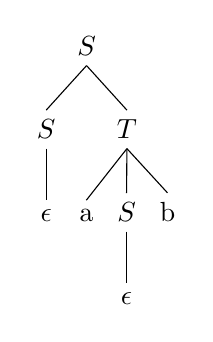
\begin{tikzpicture} \Tree
[.$S$
  [.$S$ $\epsilon$ ]
  [.$T$ a [.$S$ $\epsilon$ ] b ]
]
\end{tikzpicture}\\
6. Flemme.

\paragraph{Engendrer les langages}~\\
$L_1=L(G_1)$ avec $P_1 = (S\rightarrow\ct{a}S+\ct{a})$.\\
$L_2=L(G_2)$ avec $P_2 = (S\rightarrow AB, A\rightarrow\ct{a}A+\ct{a}, B\rightarrow\ct{b}B+\ct{b})$.\\
$L_3=L(G_3)$ avec $G_3$ comme $G_2$ sauf une règle : $A\rightarrow\ct{a}A+\epsilon$.\\
$L_4=L(G_4)$ avec $P_4 = (S\rightarrow\ct{aa}S+\ct{ab}S+\ct{ba}S+\ct{bb}S+\epsilon)$.\\
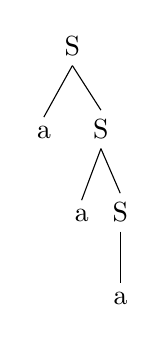
\begin{tikzpicture} \Tree
[.S a [.S a [.S a ] ] ]
\end{tikzpicture}~~~~
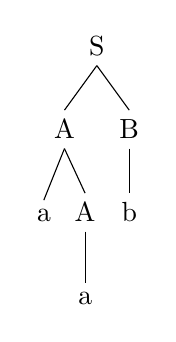
\begin{tikzpicture} \Tree
[.S [.A a [.A a ] ] [.B b ] ]
\end{tikzpicture}~~~~
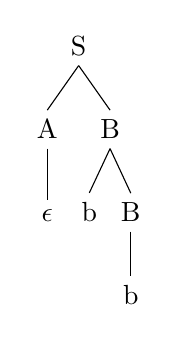
\begin{tikzpicture} \Tree
[.S [.A $\epsilon$ ] [.B b [.B b ] ] ]
\end{tikzpicture}~~~~
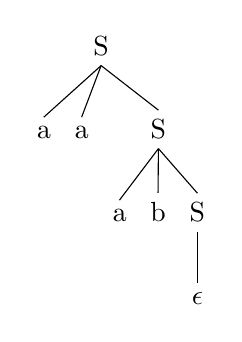
\begin{tikzpicture} \Tree
[.S a a [.S a b [.S $\epsilon$ ] ] ]
\end{tikzpicture}

\end{document}
